\section{Dual conics}

\begin{definition}[\textit{Dual conic}]
    A dual conic is a set of lines $\mathbf{l}$ that satisfy equation:
    \[\mathbf{l}^T\mathbf{C}^\ast\mathbf{l}=0\]
    where $\mathbf{C}^\ast$ is a $3 \times 3$ symmetric matrix.
\end{definition}
\begin{definition}[\textit{Non degenrate dual conic}]
    A non degenerate dual conic is a dual conic whose matrix $\mathbf{C}^\ast$ is non-singular: 
    \[\textnormal{rank}(\mathbf{C}^\ast)=3\]
\end{definition}
Consider a non-degenerate conic, denoted as $\mathbf{C}$, and the collection of all lines $\mathbf{l}$ that are tangents to it.
For each point $\mathbf{c}$ on the conic $\mathbf{C}$, there exists a line $\mathbf{l}$ that is tangent to $\mathbf{C}$. 
Since $\mathbf{l}$ is the polar line of $\mathbf{x}$ with respect to $\mathbf{C}$, we can express it as $\mathbf{l}=\mathbf{Cc}$.
Consequently, we can represent $\mathbf{x}$ as:
\[\mathbf{x}=\mathbf{C}^{-1}\mathbf{l}\]
Moreover, given that $\mathbf{C}$ is a symmetric matrix, we have:
\[\mathbf{x}^T=\mathbf{l}^T\mathbf{l}^{-T}=\mathbf{l}^T\mathbf{C}^{-1}\]
Now, considering that the point $\mathbf{x}$ lies on the conic $\mathbf{C}$, we have:
\[\mathbf{x}^T\mathbf{Cx}=0\]
By substituting the previously derived expressions, we arrive at:
\[\mathbf{l}^T\mathbf{C}^{-1}\mathbf{l}=0\]
This equation represents a quadratic homogeneous equation on $\mathbf{l}$. 
Therefore, we can conclude that for the dual conic holds $\mathbf{C}^\ast=\mathbf{C}^{-1}$. 
We can also note that a non-degenerate dual conic $\mathbf{C}^\ast$ is the collection of lines that are tangent to a non-degenerate conic $\mathbf{C}$.

\subsection{Degenerate dual conics}
\begin{definition}[\textit{Degerate dual conic}]
    A degenerate dual conic is a conic where the matrix $\mathbf{C}^\ast$ is singular: 
    \[\textnormal{rank}(\mathbf{C}^\ast) < 3\]
\end{definition}
There are two possible scenarios to consider:
\begin{itemize}
    \item When $\textnormal{rank}(\mathbf{C}^\ast) = 2$, any symmetric $3 \times 3$ matrix $\mathbf{C}^\ast$ can be expressed as:
        \[\mathbf{C}^\ast=\mathbf{pq}^T+\mathbf{qp}^T\]
        In this case, the conic represents the line $\mathbf{l}$ passing through point $\mathbf{p}$ or the line $\mathbf{l}$ passing through point $\mathbf{q}$.
        \begin{figure}[H]
            \centering
            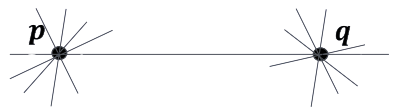
\includegraphics[width=0.35\linewidth]{images/deg2.png}
        \end{figure}
    \item When $\textnormal{rank}(\mathbf{C}^\ast) = 1$, any symmetric $3 \times 3$ matrix $\mathbf{C}^\ast$ can be expressed as:
        \[\mathbf{C}^\ast=\mathbf{pp}^T\]
        In this situation, the conic corresponds to the line $\mathbf{l}$ going through point $\mathbf{p}$ repeated twice. 
        \begin{figure}[H]
            \centering
            
\includegraphics[width=0.4\linewidth]{images/deg1.png}
        \end{figure}
\end{itemize}

\begin{definition}[\textit{Conic dual to the circular points}]
    The degenerate dual conic $\mathbf{C}^\ast=\mathbf{pq}^T+\mathbf{qp}^T$ going through two circular point $\mathbf{p}$ and $\mathbf{q}$ is known as the conic dual to the circular points, and it can be expressed as:
    \[\mathbf{C}^\ast_{\infty}=\mathbf{IJ}^{T}+\mathbf{JI}^{T}=
    \begin{bmatrix}
        1 & 0 & 0 \\
        0 & 1 & 0 \\
        0 & 0 & 0 
    \end{bmatrix}\]
\end{definition}